 \subsection{Mixtures of Gaussians}

Mixtures of Gaussian or the Gaussian Mixture Model (GMM) is a method of clustering data that's able to disentangle ambiguous samples by considering a sample's probability of belonging to a class, known as a soft assignment. 

Initially, K Gaussian functions are randomly generated corresponding to K clusters. If a dataset has low dimensionality, by taking a histogram of its values the Gasussians' initial conditions can be approximated, as in Figure \ref{fig:histGauss}. By superpositioning all of the Gaussians a sample's complete probabilistic model is created, i.e. a model for \emph{all} clusters, see Figure \ref{fig:histCurve}. 

\begin{figure}[H]
	\centering
	\begin{subfigure}[b]{0.5\linewidth}
            \centering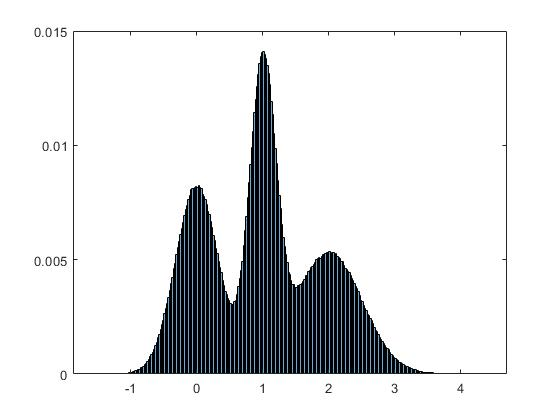
\includegraphics[width=215pt]{histGauss}
      		\caption{Normalized Histogram of 1D samples.}
		\label{fig:histGauss}
    	\end{subfigure}%
    	\begin{subfigure}[b]{0.5\linewidth}
      		\centering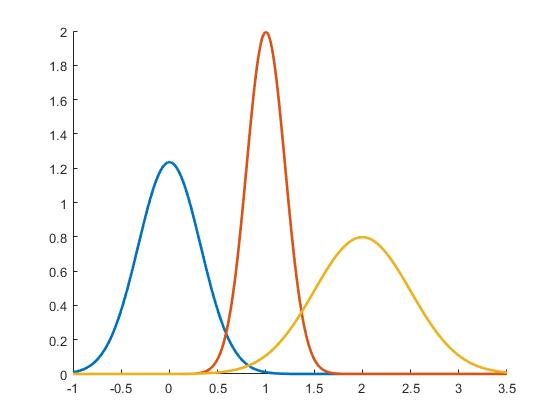
\includegraphics[width=215pt]{hist_gauss_curve}
      		\caption{Gaussians derived from 1D histogram.}
       		\label{fig:histCurve}
		\end{subfigure}
		\caption{Formulation of Mixture of Gaussians.}
    	\label{fig:mixture}
\end{figure}

With each iteration of the GMM algorithm the parameters of the model's component Gaussians are tuned according to the covariance between samples in each cluster. In \ref{eq:cov} $X$ and $Y$ are the variables being compared, $\overline X$ and $\overline Y$ are variable means and $n$ is the number of samples. For a multidimensional dataset a covariance matrix $\bm{\Sigma_k}$ will be generated and each Gaussian will require a mean vector $\bm{\mu_k}$ as opposed to a scalar. 

\begin{equation}
Cov(X, Y) = \frac{\Sigma(X_i-\overline X)(Y_j-\overline Y)}{n}
\label{eq:cov}
\end{equation}



The algorithm seeks the highest covariance possible in each of its clusters. It is by considering the covariance of samples that the GMM is able to best classify ambiguous samples. The higher the covariance (aka correlation) between sample dimensions the more likely it is they belong in the same cluster. This can observed in Figure \ref{fig:mogcov}, the data being clustered is the same as in Figure \ref{fig:clusters} but notice the elliptical shape of the Gaussian cluster distributions as opposed to the spherical shape of K-Means clustering.

\begin{figure}[H]
	\centering
	\centering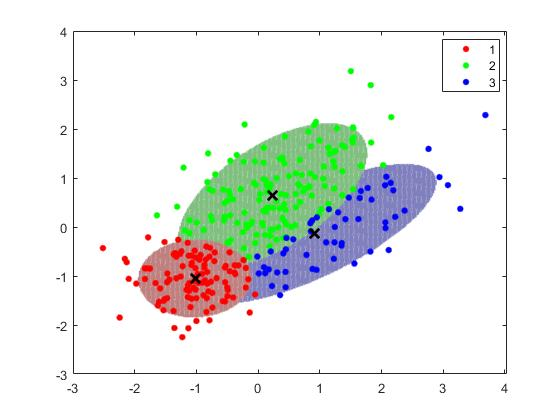
\includegraphics[width=450pt]{mog}
	\caption{Clustering using GMM. X marks cluster mean.}
	\label{fig:mogcov}
\end{figure}
  
In Figure \ref{fig:histScale} the Gaussians from Figure \ref{fig:histCurve} have been scaled to have the amplitudes $\pi_1 = 0.3$, $\pi_1 = 0.5$ and $\pi_1 = 0.2$. These are weightings that give the mixing ratio of the GMM and represent each cluster's proportion of the total samples. The more samples a cluster contains the more likely it is a sample belongs to it. The sum of ratios must add to one because the probability a sample belongs to at least one cluster is one, as defined in \ref{eq:gauss_weight1} and \ref{eq:gauss_weight2}.

\begin{equation}
    0\leq \pi_k \leq 1
\label{eq:gauss_weight1}
\end{equation}
\begin{equation}
    \sum_{k=1}^{K}\pi_k = 1
\label{eq:gauss_weight2}
\end{equation}


\begin{figure}[H]
    \centering
    \centering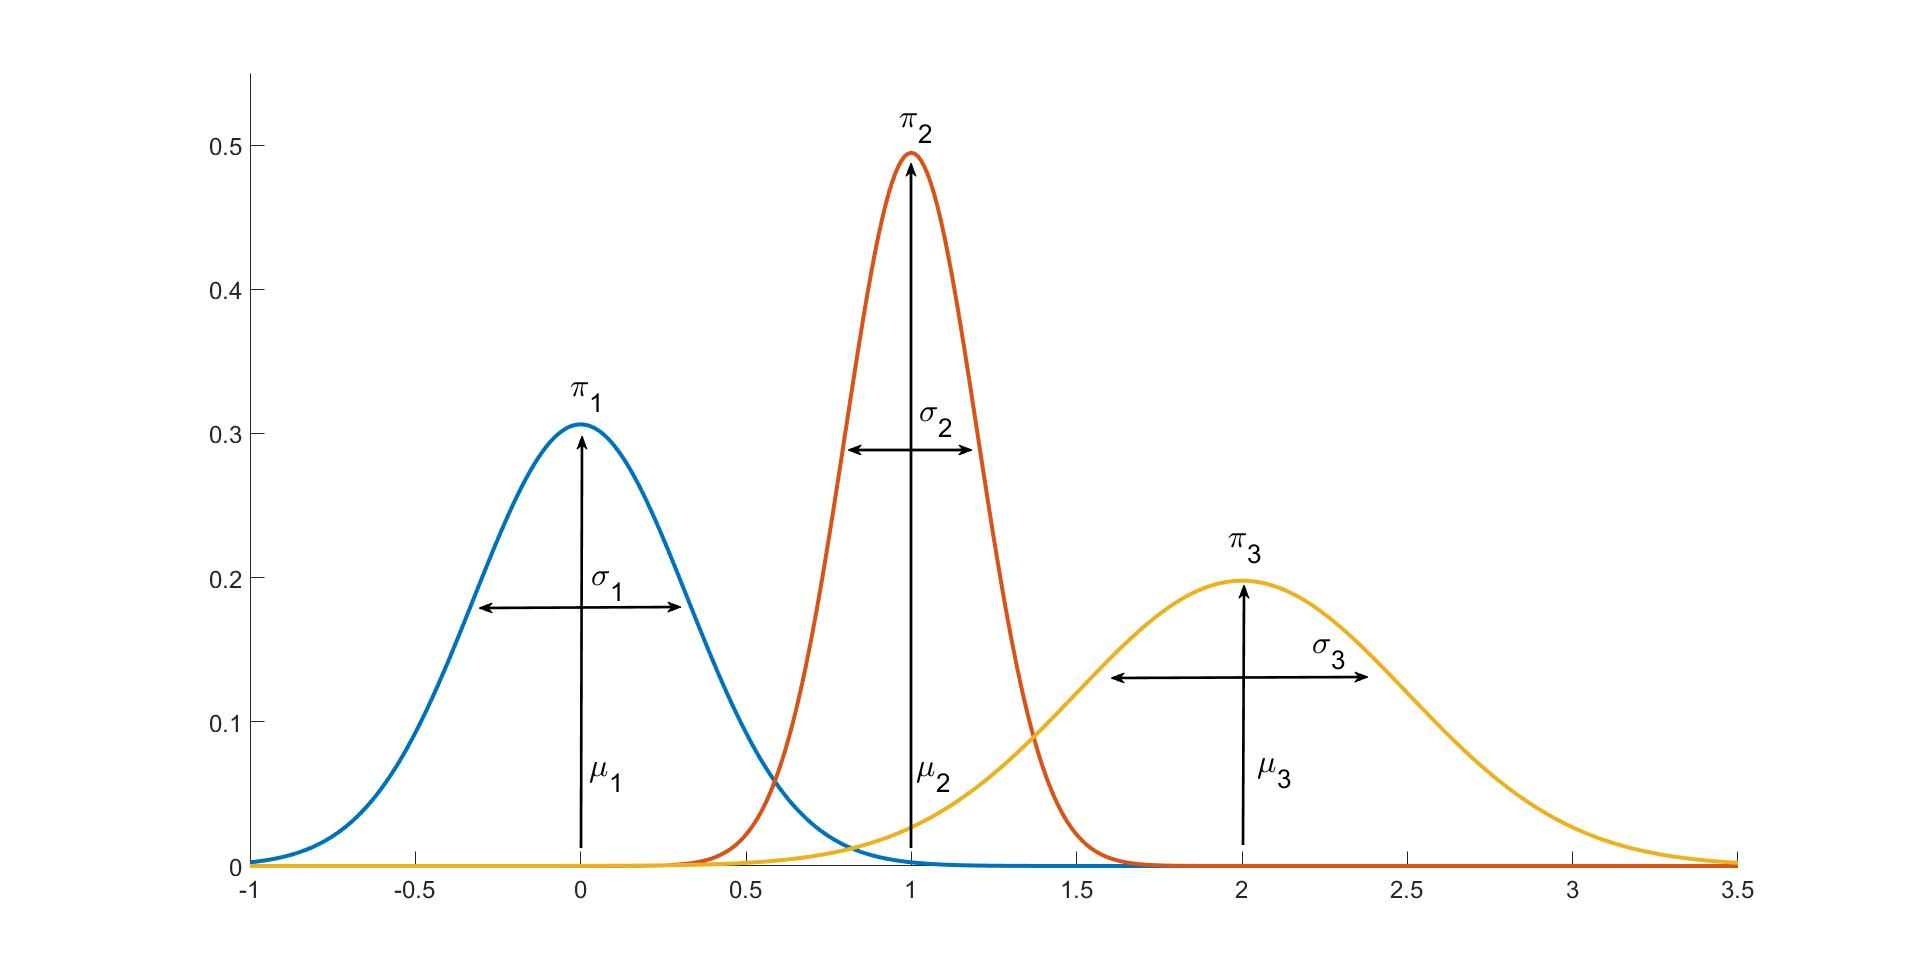
\includegraphics[width=450pt]{gauss_mix_scale}
    \caption{Individual Gaussians with scaled weightings.}
    \label{fig:histScale}
  \end{figure} 

Each Gaussian's three parameters, mean $\bm{\mu}_k$, ampltidue $\pi_k$ and covariance $\bm{\Sigma}_k$ are updated following each iteration of the algorithm according to the 'Expectation Maximization' algorithm.

\subsubsection{Expectation Maximization}

Expectation Maximization (EM) is a method of updating the parameters of cluster Gaussians that seeks to maximize a sample's likelihood of belonging to said Gaussians (\ref{eq:likelihood}). 

\begin{equation}
\label{eq:likelihood}
p(x) = \sum^K_{k=1} \pi_k \mathcal{N}(x|\bm{\mu}_k, \bm{\Sigma}_k)
\end{equation}

A binary indicator $z_{i}$ exists for every sample $x_i$, it is 1 if the sample belongs in the cluster $k$ and 0 otherwise such that $z_{ik} \in \{0, 1\}$ and $\sum_k z_{ik} = 1$. If the data is multidimensional then the sample and inidicator are both vectors, $\bm{x}$ and $\bm{z}$. The marginal probability $p(\bm{z}_{k} = 1)$ is the probability that a sample $\bm{x}$ is in cluster $k$. This quantity is completely specified by the mixture weight $\pi_k$ for each Gaussian because the area under a Gaussian component is equal to its mixing ratio, i.e.

\begin{equation}
	\label{eq:marginalk}
	p(\bm{z}_{k}=1) = \pi_k 
\end{equation}
	
If we know that a sample $\bm{x}$ is from cluster $k$ the \emph{likelihood} of seeing it in the associated Gaussian is the value of the Gaussian at that point,
\begin{equation}
	\label{eq:cond}
	p(\bm{x}\, |\, \bm{z}_{k} = 1) = \mathcal{N}(\bm{x}\, |\,\bm{\mu_k}, \bm{\Sigma_k})
\end{equation}

The conditional probability of $\bm{z}_{ik}$ given the value of sample, $\bm{x}_i$ is denoted as $\gamma(\bm{z}_{ik})$. This is the probability that a sample belongs to cluster $k$ given its value $\bm{x}_i$ and is the quantity of interest when trying to classify a sample.  Using Bayes Theorem [REF APPENDIX] quantity can be found 

\begin{align}
	\gamma(\bm{z}_{ik}) \equiv p(\bm{z}_{ik} =1 | \bm{x}_i)
	\label{eq:gamma2}
	&= \frac{p(\bm{z}_{ik}=1)p(\bm{x}_i\, |\, \bm{z}_{ik} = 1)}{\sum^K_{j=1}p(\bm{z}_{jk}=1)p(\bm{x}_j\, |\, \bm{z}_{jk} = 1)}\\ 
	\label{eq:gamma3}
	&= \frac{\pi_k\, \mathcal{N}(\bm{x}\,|\,\bm{\mu_k},\bm{\Sigma_k})}{\sum_{j=1}^{K}\pi_k\, \mathcal{N}(\bm{x}\,|\,\bm{\mu_k},\bm{\Sigma_k})}
\end{align}


To maximize the likelihood of each sample being in each Gaussian the distribution parameters are modified. This is achieved by taking derivatives of the log of the likelihood function (\ref{eq:likelihood}) with respect to each Gaussian parameter and setting the result to 0 to find local maxima. To take the log of the likelihood function assume all samples in are in an $N \times D$ matrix $\bm{X}$ and the corresponding indicators are in an $ N \times K$ matrix $\bm{Z}$. 

\begin{equation}
\label{eq:log}
ln\,p(X|\bm{\pi}, \bm{\mu}, \bm{\Sigma}) = \sum_{n=1}^N
ln \Bigg\{ \sum_{k=1}^K \pi_k\mathcal(N)(\bm{x}_n|\bm{\mu}_k,\bm{\Sigma}_k)\Bigg\}
\end{equation}







\centerline{}

The EM algorithm is comprised of [X] steps

%% EM STEPS %%
\begin{enumerate}
	\item Generate the initial K Gaussian parameters mean $\bm{\mu}_{k}$, covariance $\bm{\Sigma}_k$ and mixing ratios $\pi_k$ either randomly or informed by a histogram.
	\item Estimate the likelihood sample n was generated by cluster k for all samples. 
	\begin{equation}
		\gamma(\bm{z}_{ik})=\frac{\pi_k\, \mathcal{N}(\bm{x}\,|\,\bm{\mu_k},\bm{\Sigma_k})}{\sum_{j=1}^{K}\pi_k\, \mathcal{N}(\bm{x}\,|\,\bm{\mu_k},\bm{\Sigma_k})}
	\end{equation}

	\item Maximize the Gaussian parameter using derivatives of log likelihood for each parameter.
	\begin{align}	
	\label{eq:mean}
	\bm{\mu}_{k}^{new} &= \frac{1}{N_k}\sum_{n=1}^N \gamma(z_{nk} ) \bm{x}_n \\
	\label{eq:covariance}
	\bm{\Sigma}_k^{new} &=  \frac{1}{N_k}\sum_{n=1}^N\gamma(z_{nk})(\bm{x}_n- \bm{\mu}_k^{new})(\bm{x}_n - \bm{\mu}_k^{new})^T \\
	\label{eq:ratio}
	\pi_k &= \frac{N_k}{N}
	\end{align}
	where \newline
	\[N_k = \sum_{i} z_{ik}\]
	\item Repeat steps 2 and 3 until convergence of log likelihood (\ref{eq:likelihood}) or parameters. 
\end{enumerate}

